% Name: Subplots with groupplots
% Description: Four small plots in a 2 by 2 grid that share their size and style.
% Tags: subplots, groupplots, multiple axes

\usepackage{pgfplots}
\usepgfplotslibrary{groupplots}
\pgfplotsset{compat=1.18}

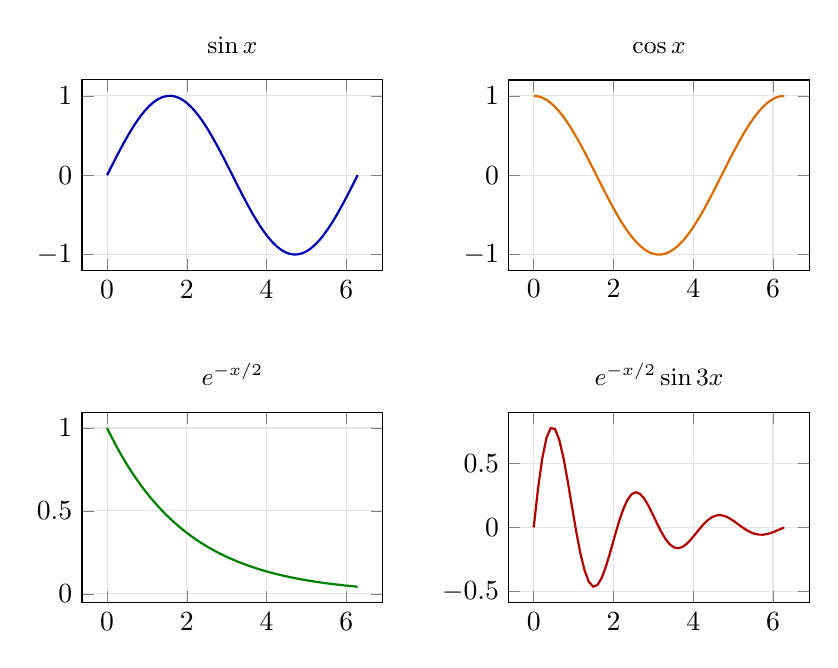
\begin{tikzpicture}
  \begin{groupplot}[
    group style={group size=2 by 2, horizontal sep=1.6cm, vertical sep=1.8cm},
    width=5.4cm, height=4cm, domain=0:2*pi, samples=60,
    grid=major, grid style={gray!20}, title style={font=\small},
  ]
    \nextgroupplot[title={$\sin x$}]
      \addplot[blue!70!black, thick] {sin(deg(x))};
    \nextgroupplot[title={$\cos x$}]
      \addplot[orange!85!black, thick] {cos(deg(x))};
    \nextgroupplot[title={$e^{-x/2}$}]
      \addplot[green!50!black, thick] {exp(-x/2)};
    \nextgroupplot[title={$e^{-x/2} \sin 3x$}]
      \addplot[red!70!black, thick] {exp(-x/2)*sin(deg(3*x))};
  \end{groupplot}
\end{tikzpicture}
